\chapter{Implementazione del sistema}

\section{Architettura}
%prova a definire gli use case con una tabella, in generale espandi questa parte.
L’architettura proposta è di tipo event-driven, per cui il processamento dei dati avviene solo quando si verifica una situazione particolare sull’edge, dato il seguente scenario: uno o più operatori entrano all’interno di una certa area definita da un insieme di ancore, su cui sono montati dei sensori e si trovano in prossimità di un macchinario attivo; due telecamere, una superiore ed una frontale monitorano l’area di sicurezza. Se almeno uno degli operatori non possiede i dispositivi di sicurezza, il sistema deve generare un allarme e spegnere il macchinario. Lo stesso tipo di reazione deve verificarsi se almeno uno degli operatori non è abilitato ad operare sulla macchina. Infatti, coloro che possono lavorare indossano un tag attivo che trasmette informazioni ai sensori sulle ancore.

\begin{figure}[htbp]
    \centering
    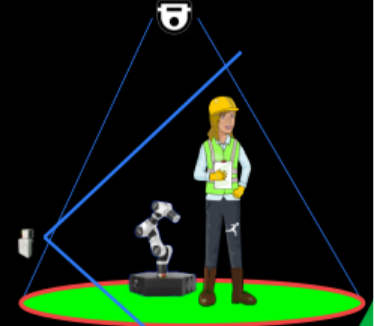
\includegraphics[width=0.5\textwidth]{figures/use-case.png}
    \caption{Schema dello use case.} 
    \label{use-case}
\end{figure}


 Il design è quello di un’ applicazione cloud nativa e si divide in due sottosistemi tra di loro connessi: da un lato l'edge, composto da una telecamera superiore accoppiata ad una frontare, dei sensori ed un gateway; dall'altro il cloud formato da servizi gestiti dal provider AWS. Il progetto non è una classica applicazione client-server, ma un insieme di servizi gestiti che globalmente opera near-real time e si serve di dispositivi IoT sia per la rilevazione degli eventi che per l’ingestion dei dati sul cloud. Nel primo caso viene utilizzato MQTT per la telemetria. Nel secondo invece, vengono connesse le telecamere ad un gateway attraverso il protocollo RTSP e successivamente questo si occupa dell'ingestion effettiva, sfruttando una libreria Amazon apposita. 

\begin{figure}[htbp]
    \centering
    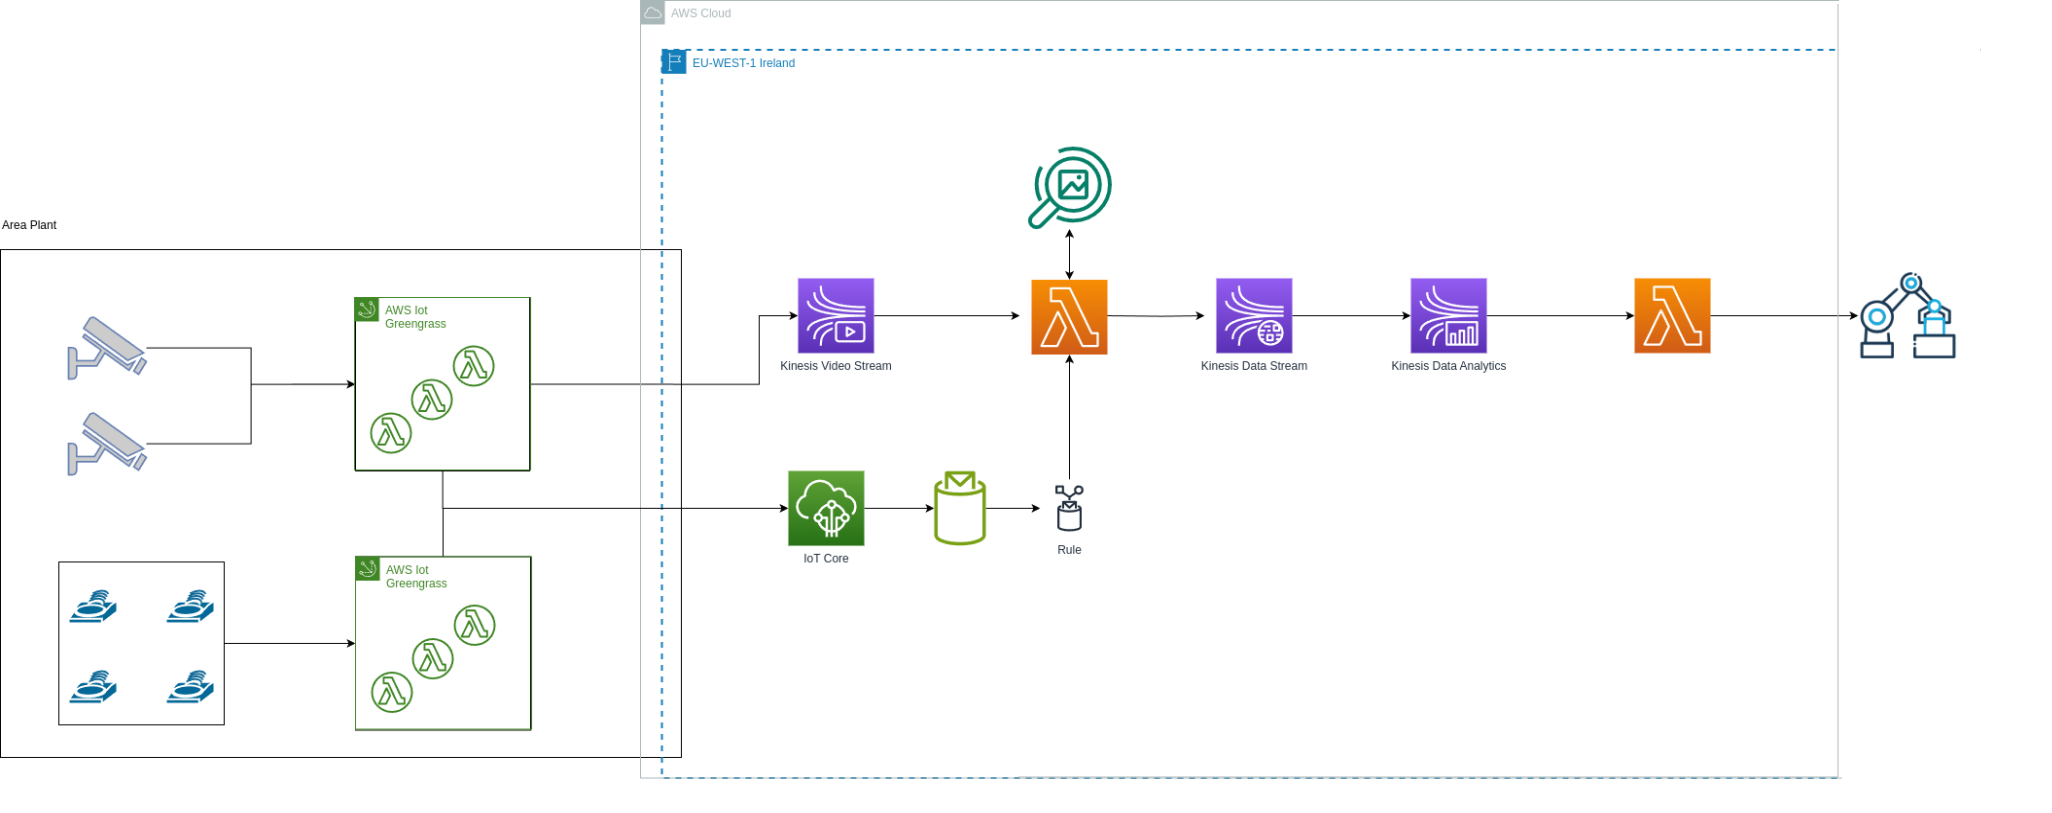
\includegraphics[width=0.85\textwidth]{figures/architettura.png}
    \caption{Architettura ad alto livello del sistema.} 
    \label{fig:architettura}
\end{figure}
 

Il gateway posto tra i dispositivi e il cloud non serve solo per garantire la necessaria potenza di calcolo per l’invio dei dati, ma è un componente imprescindibile per l’integrazione con AWS. Al suo interno infatti è installato un software fondamentale per la realizzazione del sistema: IoT Greengrass. Una delle sue funzionalità più importanti è quella di installare sull'edge componenti software caricati dal cloud. Esso consente uno sviluppo del progetto molto più rapido e semplice, consen. Si occupa di problemi come: 


\begin{itemize}
	\item \textbf{sicurezza sull’edge e dei dati in transito}: Greengrass è installato con permessi di root e sfrutta le user permission per l’anti-tampering del codice dopo il deploy. Per la comunicazione in entrata ed uscita, si serve di certificati relativi alla public key infrastructure (PKI) rilasciati da aws. Per cui, tramite autenticazione, cifratura e integrità dei dati sia la comunicazione che i deploy sono sicuri di default.
	\item \textbf{orchestrazione del runtime}: i componenti che vengono deployati dal cloud verso l’edge, in qualsiasi forma essi siano (monoliti, servizi o container) possono essere gestiti dall’ambiente in modo da definire dipendenze tra i vari componenti ed un lifecycle per ciascuno di essi.  
	\item \textbf{logging e monitoraggio}: questa integrazione è fondamentale soprattutto per dispositivi che non sono facilmente accessibili da remoto. I log generati dai componenti possono essere automaticamente sincronizzati con servizi cloud aws come cloudwatch. Inoltre lo stato dei dispositivi è automaticamente tracciato in modo tale da controllare quelli che riscontrano dei problemi e rispondere rapidamente agli errori.
	\item \textbf{scalabilità del deployment}: con Greengrass possono essere definiti gruppi di dispositivi su cui deployare dei componenti. Un dispositivo può appartenere anche a più gruppi e può quindi ricevere diversi deployment contemporaneamente. La definizione di questi insiemi permette quindi un controllo granulare delle istanze per le quali serve fare merging di diversi deployment.
\end{itemize}

L'obiettivo di questi primi paragrafi è quello di descrivere i componenti hardware e software sull’edge ed i servizi gestiti sul cloud che si occupano dell’ingestion dei dati in maniera sicura, robusta e scalabile, con accenni sulla trasformazione e il preprocessamento dei dati(vedi Figura \ref{fig:sub-ing}). In questa soluzione, Greengrass è installato all’interno di un container Docker che ha come immagine di base la più recente versione di Amazon Machine Image (AMI), pensata per essere integrata con AWS e quindi essere più efficiente e sicura all’interno dell’infrastruttura cloud. Questa macchina virtuale è stata customizzata in modo da supportare sia le dipendenze di Greengrass, che quelle per GStreamer, un tool per l’inoltro dello streaming, che collabora con la libreria apposita per l'invio sul cloud. L’ingestion dei dati video e di quelli provenienti dai sensori è separato ed avviene in due modalità differenti. Una volta che il componente video viene deployato inizia ininterrottamente a streammare su KVS, mentre il publisher che genera l’evento, inviandolo ad un broker su AWS IoT, si attiva solamente alla rilevazione da parte dei sensori di uno o più operatori. 

Attraverso Greengrass è possibile generare lo stesso runtime che sul cloud permette l’esecuzione di uno dei componenti più noti in AWS, cioè Lambda, una funzione gestita direttamente dal provider, che elimina la necessità di configurazione di macchine virtuali, sistemi operativi e scalabilità. Il tutto avviene nell’ottica di concentrarsi solo sullo sviluppo della logica per la reazione agli eventi. In questo modo i sensori pubblicheranno i dati su una coda MQTT locale, come il numero di tag rilevati o la macchina cui si fa riferimento, e successivamente la Lambda sull'edge, iscritta al relativo topic, si attiverà alla pubblicazione di queste informazioni. Una volta eseguita una prima elaborazione, la funzione pubblicherà su un topic in IoT Core, generando un evento in formato JSON. 

\begin{figure}[htbp]
    \centering
    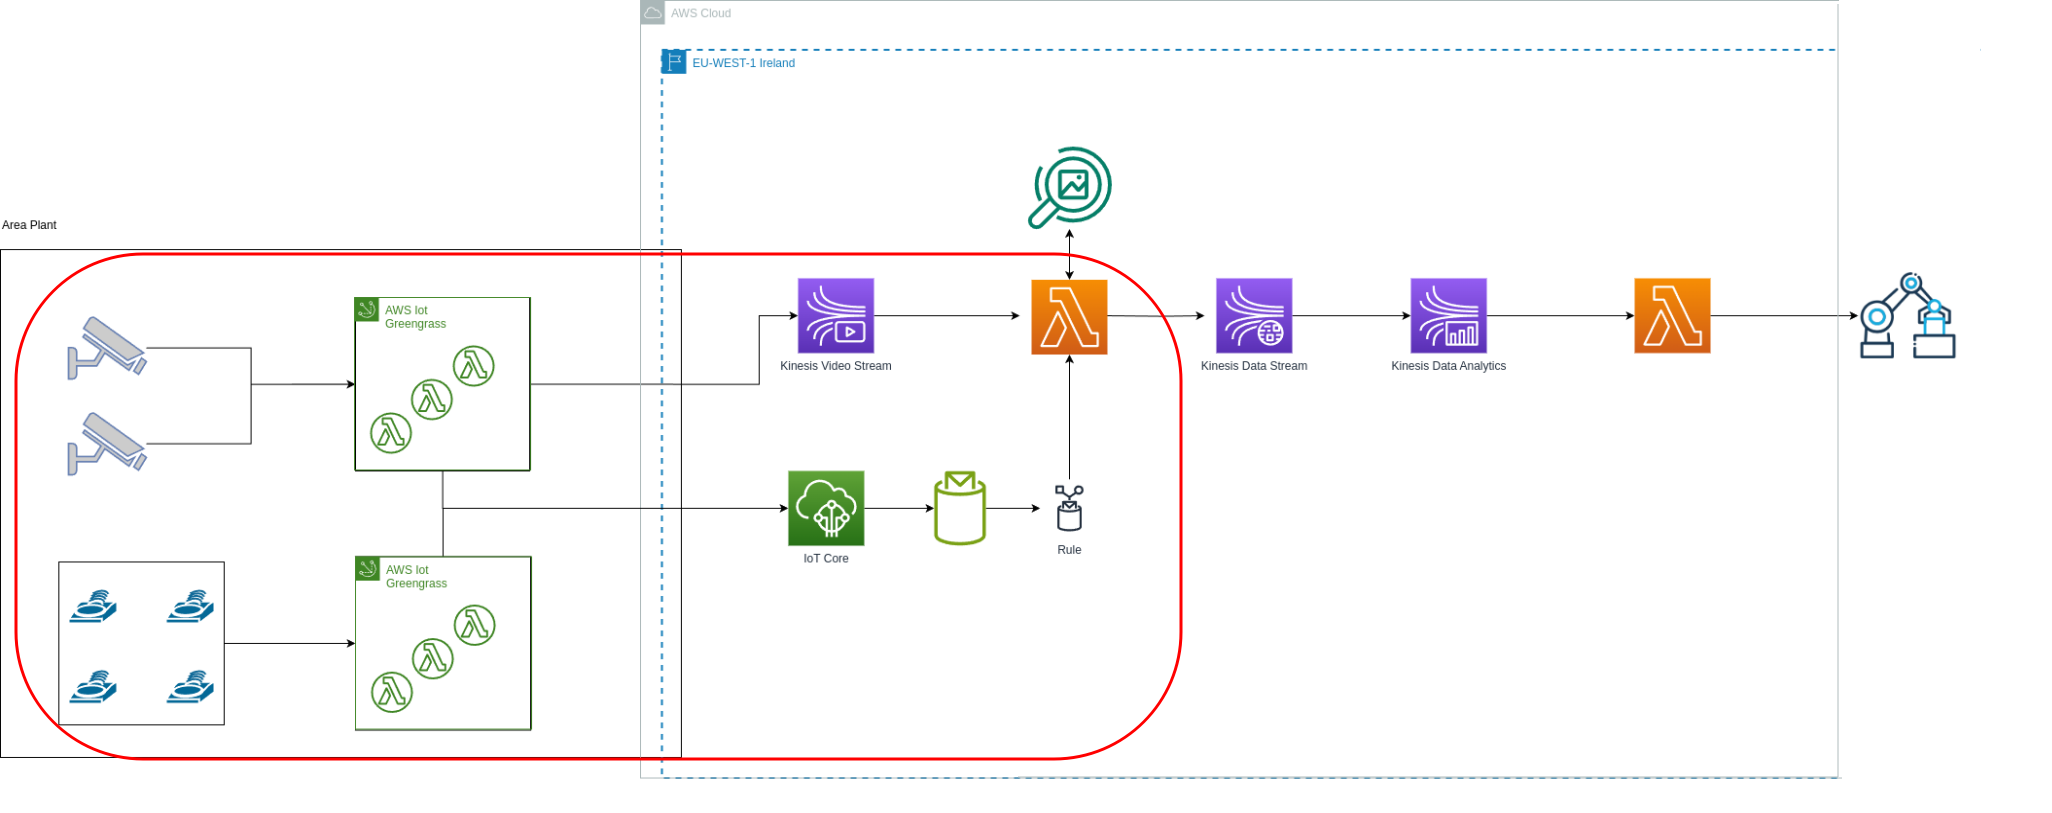
\includegraphics[width=0.85\textwidth]{figures/sottosistema-ingestion.png}
    \caption{Sottosistema di ingestion e preprocessing.} 
    \label{fig:sub-ing}
\end{figure}

Al messaggio MQTT vengono applicate delle regole, in modo tale da filtrare i dati, successivamente trasmessi ad un’altra Lambda che si trova sul cloud, la quale si occupa del processamento dello streaming video. A valle dell’analisi viene prodotto uno stream di dati verso un’applicazione big data. Nel dettaglio, il flusso iniziale viene separato in due, in quanto la Lambda è progettata per elaborare uno streaming video alla volta ed i flussi streaming da analizzare in parallelo provengono, come già visto, da una telecamera frontale e una superiore. Per cui ogni evento che triggera la Lambda deve contenere un riferimento allo stream: in questo modo, contemporaneamente, due istanze diverse della stessa Lambda verranno attivate a valle del topic filter. 

Per concludere il quadro della descrizione architetturale, bisogna focalizzarsi sui dati in uscita dalla Lambda. Ogni frame analizzato dallo streaming video viene inviato in modalità asincrona sul servizio gestito Kinesis Data Stream (KDS), il quale permette la trasmissione di grandi flussi di dati in real-time. Queste informazioni possono essere successivamente analizzate in parallelo su dei cluster, dopo aver deployato una opportuna applicazione big data. Si tratta quindi del centro di elaborazione all'interno dell'architettura, in quanto è il punto in cui tutti gli eventi vengono uniti dalle diverse sorgenti IoT, che siano le telecamere o i sensori. In questo progetto è stata sviluppata una applicazione con Apache Flink, come già visto nel capitolo precedente, il framework e motore di processamento distribuito per flussi di dati streaming sia limitati che illimitati. 
%rivedi questa parte
A differenza di altre soluzioni, come Apache Spark, questo framework non solo supporta il batching, ma anche l’analisi di singoli record provenienti da un flusso di dati real-time. Amazon offre un servizio gestito per l’analisi chiamato Kinesis Data Analytics, ma per gli esempi e la ridotta scala dei dati è stato scelto di deployare l’applicazione su una istanza EC2. Il risultato è equivalente e il codice non deve essere modificato per funzionare su un eventuale cluster. Infine, all'estremo del sistema è presente un'ultima Lambda, la cui responsabilità è quella di restituire gli allarmi generati in fase di processamento. 

\begin{figure}[htbp]
    \centering
    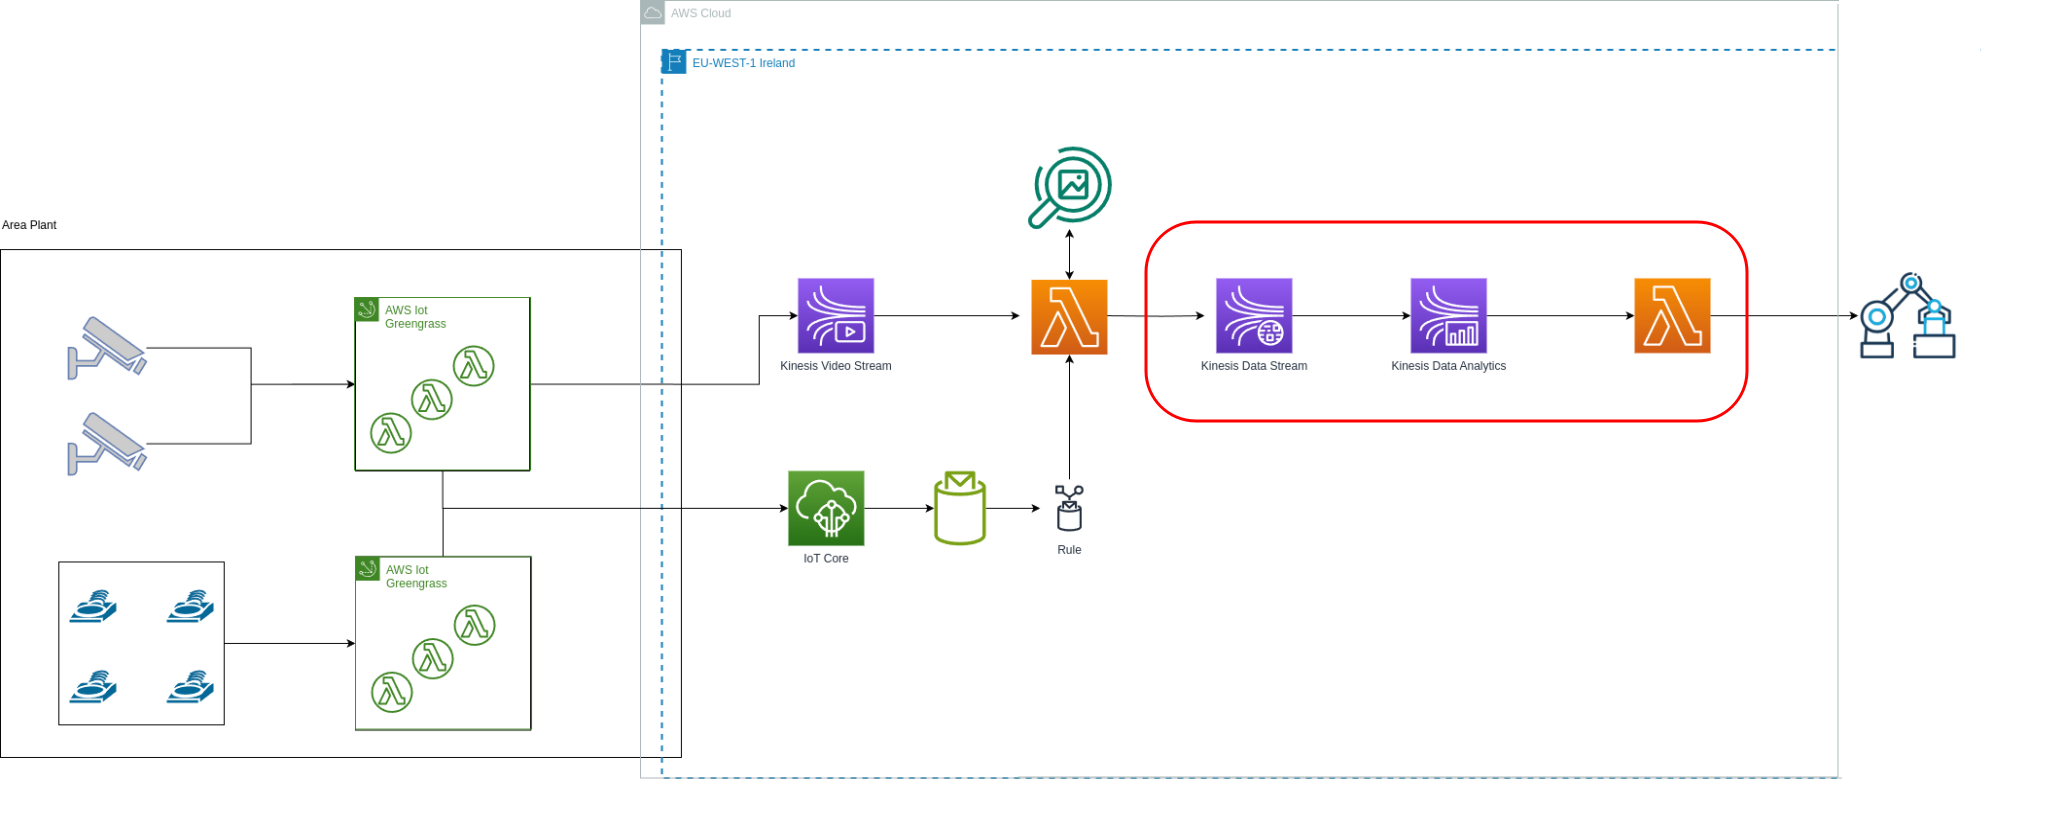
\includegraphics[width=0.85\textwidth]{figures/processing-subsystem.png}
    \caption{Moduli di processamento e generazione degli allarmi.} 
    \label{fig:processing-subsystem}
\end{figure}

\section{Edge Runtime/Ingestion}
\section{Preprocessing e trasformazione dei dati}
La parte di preprocessing, come visto nella descrizione generale, avviene tramite il coordinamento di diversi managed services, il cui fulcro è la funzione Lambda. Essa implementa la trasformazione dello streaming video in uno flusso di dati in tempo reale, integrando vari servizi AWS in maniera scalabile, efficiente e soprattuto automatica, in base al numero di stream ricevuti. I servizi utilizzati all'interno della Lambda sono Kinesis Video Streams (KVS), Amazon Rekognition, Kinesis Data Streams ed opzionalmente S3. La funzione è implementata in Python e sfrutta internamente il multithreading per l'ottimizzazione delle prestazioni. Alla base di questo sistema c'è il \texttt{lambda\textunderscore handler}, i.e. l'entryponit del codice, invocato all’arrivo di un nuovo evento. In termini più specifici, questo tipo di attivazione prende il nome di trigger e viene generato attraverso una topic rule, un meccanismo di filtro fornito da IoT Core. Poiché si tratta del payload di un messaggio MQTT, l'evento viene inviato sotto forma di JSON. Il filtro esegue quindi due operazioni: in primo luogo verifica che il topic sia quello di interesse della Lambda; successivamente può modificare il contenuto del messaggio, scartando alcuni campi, in base a come è stata definita la regola sul servizio. In generale, nella maggior parte dei casi, la comunicazione dei componenti all'interno del cloud è completamente trasparente all'utente e molti servizi non necessitano dell'invocazione diretta delle API, come invece capita normalmente nelle architetture a microservizi. La gestione viene delegata internamente all'infrastruttura AWS. Nelle parti in cui invece l'utente deve scrivere codice, la situazione è diversa: AWS in questo caso fornisce gli SDK in base al linguaggio di programmazione scelto. Nell'implementazione della funzione Lambda si sfrutta la libreria botocore per invocare le API di Rekognition e KDS.

L'algoritmo della Lambda, chiamata Kinesis Video Consumer, inizialmente si occupa di ricevere l'evento, contente il nome del flusso video da processare. Questo dato viene estratto e validato: se mancante, la funzione registra un errore e termina prematuramente. Successivamente viene stabilita una connessione con KVS, per ottenere l'endpoint da cui scaricare il flusso video. A questo punto viene creato un client apposito per accedere ai dati tramite l'API di KVS \texttt{get\textunderscore media}, agganciandosi allo stream da un momento specifico, definito tra le opzioni della chiamata. Poiché l'obiettivo del sistema è quello di elaborare un flusso in tempo reale, questo parametro deve essere impostato sul frame corrente, cioè l'ultimo che è stato caricato nel servizio KVS. Dopo il collegamento all'endpoint e l'inizializzazione del flusso, inizia l'elaborazione del video vera e propria. Lo stream viene processato iterativamente, elaborando i frammenti ricevuti dal KVS. %vedi se riesci a spiegare la logica di frammentazione.
Questa unità contiene al suo interno un certo numero di frames, il cui valore è configurabile dalla sorgente del flusso multimediale %vedi se riesci a parlare della codifica. "e.g. e come si vedrà più o avanti o come si è visto prima questo valore può impattare sulla latenza"
I relativi bytes vengono progressivamente accumulati in un buffer temporaneo, per raggiungere il confine di separazione tra un pezzo di video ed un altro. Una volta che il fragment è stato ricostruito, vengono estratti i frames contenuti al suo interno. Essi vengono successivamente codificati in un formato accettabile per la API di Rekognition. 


A questo punto ciascun frame viene inviato al servizio per l'analisi delle immagini, in particolare si sfrutta \sloppy\texttt{detect\textunderscore protective\textunderscore equipment}\fussy, specificando il tipo di DPI da rilevare ed una soglia di confidenza minima. Le chiamate avvengono in parallelo sfruttando il thread pooling, con la relativa struttura dati inizializzata prima dell'esecuzione dell'handler. Le variabili globali definite all'interno della Lambda infatti, permettono di conservare lo stato delle informazioni ad ogni nuova esecuzione della funzione, quindi al verificarsi di un nuovo evento. Quando possibile, è estremamente utile usare questo meccanismo in modo tale da ridurre al massimo il tempo di esecuzione. Inoltre, sempre in termini di efficienza, occorre che i trigger si attivino almeno ogni 15 minuti, in modo tale che non ci sia una deallocazione delle risorse associate alla Lambda. La frequenza degli eventi è imprevedibile, per cui ha senso programmarli al superamento di una certa soglia temporale. E' possibile implementare questa logica attraverso i timer impostati con il servizio CloudWatch. Infine, sempre in maniera asincrona, il JSON risultante dall'analisi viene inviato al servizio gestito KDS, invocando una opportuna API.




\section{Big data analysis}
L’applicazione big data è formata da classi per la modellazione dei dati in ingresso, per la rappresentazione dei dati trasformati e per la effettiva elaborazione. % Il main è contenuto all’interno di SafetyOnPlantsStreamingJob.java (//TODO: spiega perché vengono definiti jobs all’interno di un cluster; in generale dovresti fornire dettagli su come funziona il framework flink).

Il primo gruppo di classi, associato al data model, è fondamentale per la rappresentazione dei dati streaming in ingresso all’applicazione, provenienti dall’analisi del video. Il tutto è strutturato in modo da essere modulare e facilmente manutenibile sfruttando il paradigma della programmazione ad oggetti. La composizione delle classi permette la deserializzazione in runtime del JSON proveniente dall’elaborazione di Amazon Rekognition. %(il servizio gestito che contiene i modelli per la object detection), strutturato nel seguente modo:
Esse sono strutturate nel seguente modo:

\begin{itemize}
	\item \textbf{RekoResult}: È la classe principale che rappresenta il risultato di un'analisi video per la rilevazione dei dispositivi di protezione individuale. Contiene la versione del modello machine learning che ha analizzato i frame durante la fase di preprocessing, il numero totale di frame analizzati, un riepilogo dell'equipaggiamento rilevato, informazioni sulla dispositivo sorgente ed una lista di persone rilevate.
	\item \textbf{Summary}: Fornisce un riepilogo degli individui rilevati nel video, suddividendo gli identificativi in tre categorie: persone con l'equipaggiamento richiesto, senza l'equipaggiamento richiesto e con equipaggiamento indeterminato. In quest'ultimo caso il modello non è stato in grado di distinguere se un lavoratore indossasse correttamente i dispositivi.
	\item \textbf{SourceInfo}: Questa classe contiene informazioni dettagliate sulla fonte del video, quindi le informazioni sulla telecamera, l'indetificativo del sito industriale, quello del gateway e della macchina cui si sta facendo riferimento.
	\item \textbf{Camera}: Modella i dettagli della telecamera utilizzata, come l'identificativo, il tipo, lo stream video, e la telecamera associata.
	\item \textbf{Person}: Rappresenta una persona rilevata, includendo informazioni sulla posizione nel video, un elenco di parti del corpo rilevate, la confidenza del modello nella rilevazione della persona, e un idnetificativo univoco per la persona stessa.
	\item \textbf{BodyPart}: Descrive una parte del corpo di una persona rilevata, associando una confidenza nella rilevazione, e una lista di dispositivi di protezione rilevati su quella parte del corpo.
	\item \textbf{EquipmentDetection}: Rappresenta un dispositivo di protezione rilevato su una parte del corpo, con dettagli sulla posizione, il tipo di equipaggiamento, la confidenza della rilevazione, e se copre adeguatamente la parte del corpo in questione.
	\item \textbf{CoversBodyPart}: Questa classe modella il risultato dell'analisi di copertura di una parte del corpo attraverso il dispositivo di protezione. Include un valore booleano che indica la copertura e un valore di confidenza per tale rilevazione.
	\item \textbf{BoundingBox}: Utilizzata sia per le persone che per i dispositivi di protezione, questa classe definisce le coordinate di un'area rettangolare in un'immagine o video.
\end{itemize}

\begin{figure}[htbp]
    \centering
    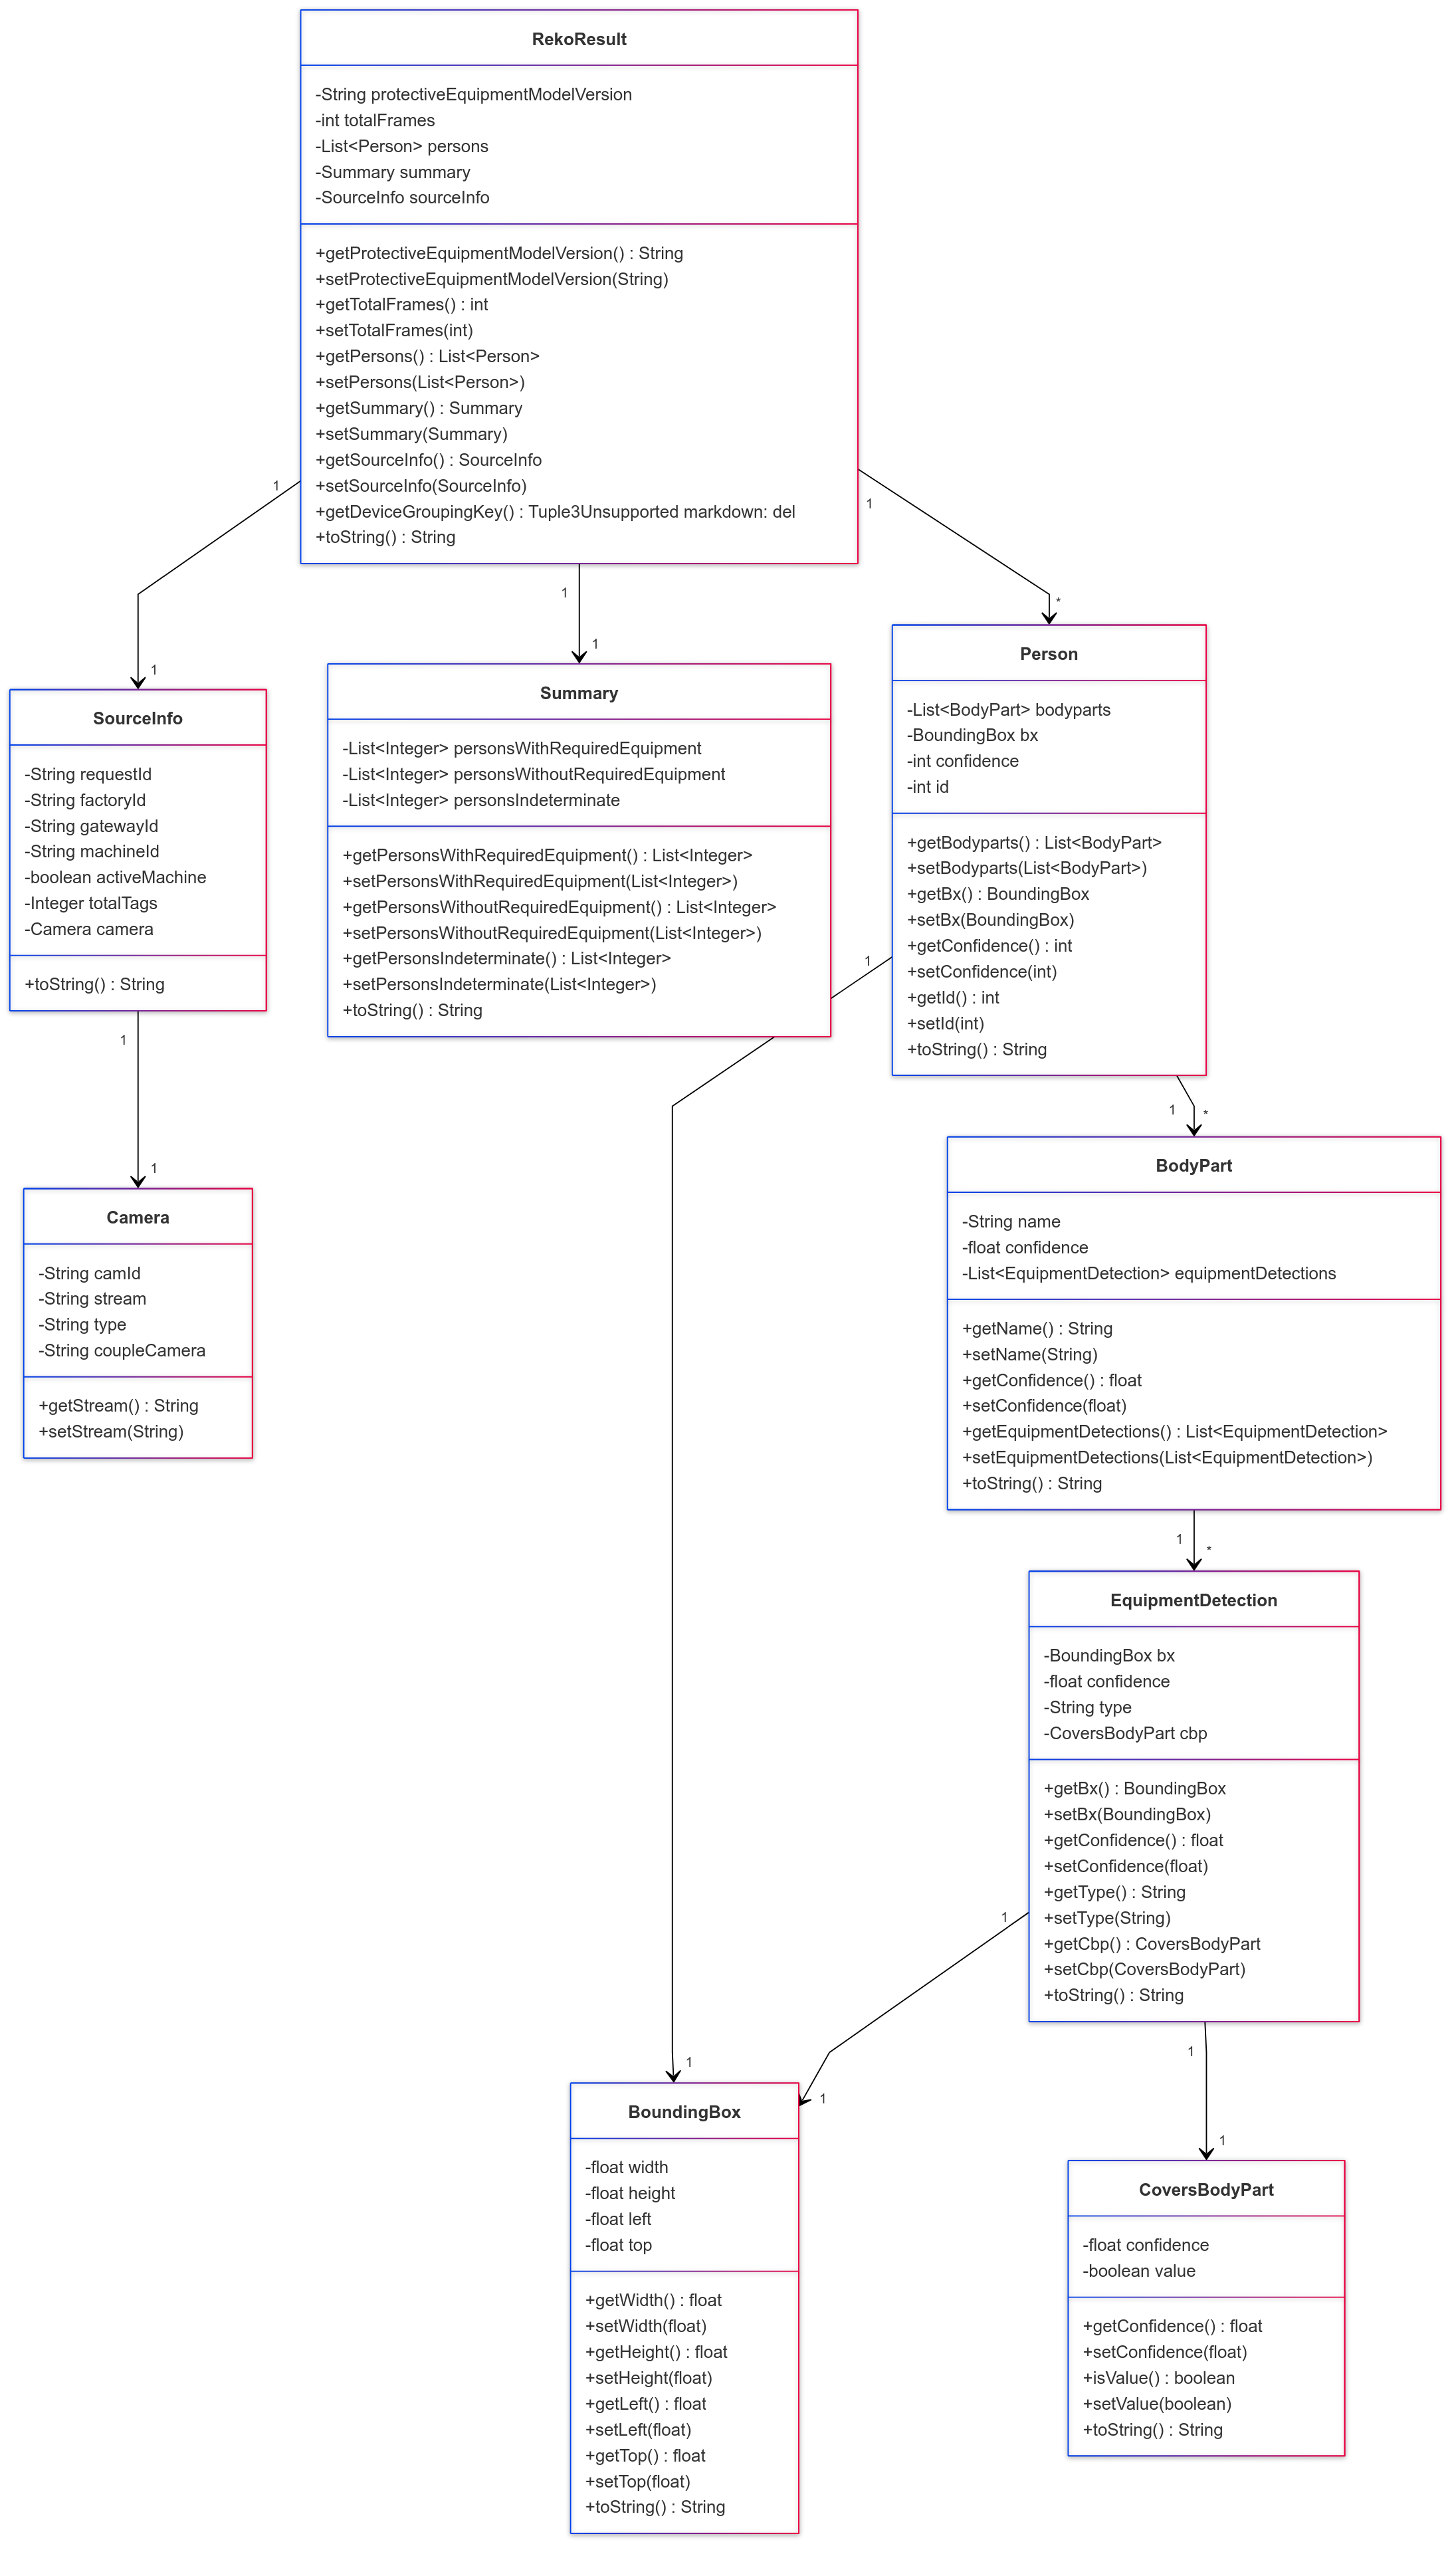
\includegraphics[width=0.47\textwidth]{figures/data-model.png}
    \caption{Diagramma modello dati.} 
    \label{fig:processing-subsystem}
\end{figure}


\section{Deployment}